\begin{figure}[t]
\centering
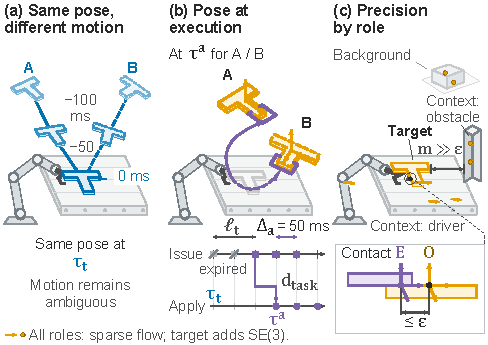
\includegraphics[width=\columnwidth]{figures/Fig3/fig3.pdf}
\caption{\textbf{Acting on a moving target} (schematic).
(a) Different histories reach the same captured pose at $\tau_t$.
(b) At the same execution time $\tau^{\mathrm a}$, target translation and rotation
differ, requiring different commands (purple). Issue slots are spaced by
$\Delta_a=50$\,ms from capture. Gray slots expire during latency $\ell_t$;
retained commands apply after task delay $d_{\rm task}$, first at
$\tau^{\mathrm a}=\tau_t+\ell_t+d_{\rm task}$.
(c) Contact aligns $E$ and $O$ within millimeter-scale $\varepsilon$; an obstacle leaves clearance
$m\gg\varepsilon$, a conveyor drives the target, and distant background does not
affect the task. Sparse flow covers all roles (arrows: displacement; dots: zero);
the target additionally receives precise SE(3) supervision.
Poses and delays are illustrative ($\ell_t=2\Delta_a$, $d_{\rm task}=\Delta_a$);
contact is enlarged.}
\label{fig:principles}
\end{figure}
